\documentclass[11pt,a4paper]{article}
\usepackage[margin=2.4cm]{geometry}
\usepackage{amsmath,amssymb}
\usepackage{graphicx}
\usepackage{booktabs}
\usepackage[font=small,labelfont=bf]{caption}
\usepackage[colorlinks=true,linkcolor=blue!60!black,citecolor=blue!60!black,urlcolor=blue!60!black]{hyperref}
\usepackage{xcolor}

\graphicspath{{figures/}{../figures/}}

% AUTO-GENERATED from results/results.json -- do not edit
\newcommand{\RefYA}{0.7158271}
\newcommand{\RefYB}{9.1855\times10^{-6}}
\newcommand{\RefYC}{0.2841637}
\newcommand{\RefDefect}{2.9\times10^{-15}}
\newcommand{\OrdEulerRob}{1.00}
\newcommand{\OrdImplRob}{1.00}
\newcommand{\OrdRKRob}{4.35}
\newcommand{\StiffOne}{3.03\times10^{3}}
\newcommand{\StiffTwo}{5.42\times10^{3}}
\newcommand{\StiffForty}{1.584\times10^{5}}
\newcommand{\LamMaxForty}{3.39\times10^{3}}
\newcommand{\HBoundEuler}{0.00059}
\newcommand{\HBoundRK}{0.00083}
\newcommand{\HCritEmp}{0.0006}
\newcommand{\SweepTableBody}{
$0.0003$ & stable (bounded) & $0$ \\
$0.0004$ & stable (bounded) & $0$ \\
$0.0005$ & stable (bounded) & $0$ \\
$0.00055$ & stable (bounded) & $0$ \\
$0.0006$ & bounded, \textbf{negative} & $-4.9\times10^{-6}$ \\
$0.0007$ & \textbf{blow-up} & -- \\
$0.0008$ & \textbf{blow-up} & -- \\
$0.001$ & \textbf{blow-up} & -- \\
}
\newcommand{\MatchedTableBody}{
Explicit Euler & $10^{2}$ & $0.00053$ & $1.9\times10^{-6}$ & 75,395 & 0.50\,s\,\,(stab.-pinned) \\
Explicit Euler & $10^{3}$ & $0.00053$ & $1.9\times10^{-6}$ & 75,395 & 0.51\,s\,\,(stab.-pinned) \\
Explicit Euler & $10^{4}$ & $0.00053$ & $1.9\times10^{-6}$ & 75,395 & 0.47\,s\,\,(stab.-pinned) \\
RK4 & $10^{2}$ & $0.00063$ & $2.6\times10^{-12}$ & 252,060 & 2.11\,s\,\,(stab.-pinned) \\
RK4 & $10^{3}$ & $0.00063$ & $2.6\times10^{-12}$ & 252,060 & 2.50\,s\,\,(stab.-pinned) \\
RK4 & $10^{4}$ & $0.00063$ & $2.6\times10^{-12}$ & 252,060 & 2.07\,s\,\,(stab.-pinned) \\
Implicit Euler & $10^{2}$ & $2$ & $0.0065$ & 93 & 0.01\,s \\
Implicit Euler & $10^{3}$ & $0.3$ & $0.001$ & 421 & 0.03\,s \\
Implicit Euler & $10^{4}$ & $0.029$ & $0.0001$ & 3,505 & 0.22\,s \\
}
\newcommand{\AdaptiveTableBody}{
$10^{4}$ & $1.2\times10^{-6}$ & 20,604 & 8,766 & 323,070 & 3.31\,s \\
$10^{5}$ & $6.1\times10^{-7}$ & 20,636 & 8,856 & 324,412 & 4.49\,s \\
$10^{6}$ & $1.2\times10^{-6}$ & 20,758 & 9,126 & 328,724 & 4.38\,s \\
}


\newcommand{\yy}{\mathbf{y}}
\newcommand{\ee}{\mathbf{e}}

\title{\textbf{Stiffness in the Robertson Chemical Kinetics System:\\
What Explicit Methods Pay, What Implicit Methods Buy}}
\author{Zihan Xu \and Beixue Liang \and Yumo Li\\[2pt]
\small Numerical Analysis of ODEs and PDEs, Project 1 (Weeks 1--4)}
\date{\today}

\begin{document}
\maketitle

\begin{abstract}
We study numerical solution of the Robertson stiff chemical kinetics system
(Classic Problem Pack, direction~\textcircled{\scriptsize 3}) on $0\le t\le 40$.  We build a small
solver library from scratch (explicit Euler, classical RK4, implicit Euler with
Newton's iteration, and an adaptive step-doubling RK4), construct our own
high-accuracy reference oracle, and answer one mathematical question:
\emph{how does stiffness --- quantified by the frozen-Jacobian eigenvalues of the
system --- translate into a practical step-size restriction for explicit methods,
and what does an implicit method pay for the same accuracy?}
Our measurements show (i) the empirical explicit-Euler stability threshold
$h\approx\HCritEmp$ agrees with the frozen-Jacobian prediction $\HBoundEuler$
to about 2\%; (ii) at a \emph{matched} error target on the full interval the
implicit method is the cheapest by one to three orders of magnitude in
right-hand-side evaluations, because the explicit methods are pinned at their
stability limits and therefore cannot trade accuracy for speed; and
(iii) adaptivity removes the accuracy constraint but \emph{not} the stability
constraint: the global error of adaptive RK4 plateaus near $10^{-6}$ as the
tolerance is tightened, because the step size is pinned at the RK4 stability
limit.  Stiffness is a stability story, and no controller can rewrite it.
\end{abstract}

\tableofcontents

%=====================================================================
\section{Background and problem choice}
%=====================================================================
Chemical reaction systems are the canonical example of \emph{stiff} initial
value problems: fast intermediate species and slow product species coexist in
one state vector, so the Jacobian of the right-hand side has eigenvalues of
very different magnitude.  The Robertson system
\cite{robertson1966} is the standard benchmark for this phenomenon: its rate
constants span eight orders of magnitude ($k_1=0.04$ vs.\ $k_2=3\times10^7$),
yet along the actual trajectory the \emph{realised} eigenvalue spread grows
over time to about $S(40)\approx\StiffForty$.

We chose direction~\textcircled{\scriptsize 3} for three reasons.
\textbf{(1) A sharp, testable question.}  The Problem Pack gives a concrete
explicit-stability estimate ($h<2/|\lambda|_{\max}\approx 5.9\times10^{-4}$ at
$t=40$) that we can compare against our own measured threshold --- a clean
falsification experiment, not just a demo.
\textbf{(2) A demanding validation story.}  Explicit methods genuinely fail
here (they oscillate, go negative, and blow up), which forces us to build
serious diagnostics: an independent oracle, invariant-plane tracking,
componentwise positivity, and a convergence-order check on the same baseline.
\textbf{(3) A lesson with a twist.}  As we show in
Section~\ref{sec:matched}, the ``obvious'' conclusion --- implicit methods win
on stiff problems --- is only true when the accuracy target is loose; the
quantitative crossover is something we measured rather than assumed.

All numbers in this report are produced by \texttt{code/run\_all.py}; every
figure regenerates from scratch in one command, and every quoted value is
stored in \texttt{results/results.json}.

%=====================================================================
\section{Model}\label{sec:model}
%=====================================================================
With $\yy=[y_1,y_2,y_3]^{\mathsf T}$ (concentrations of species $A,B,C$) the
Robertson system is
\begin{align}
y_1' &= -0.04\,y_1 + 10^4 y_2 y_3, \notag\\
y_2' &= \phantom{-}0.04\,y_1 - 10^4 y_2 y_3 - 3\times10^7 y_2^2, \label{eq:robertson}\\
y_3' &= \phantom{-}3\times 10^7 y_2^2, \notag
\end{align}
with $\yy(0)=[1,0,0]^{\mathsf T}$ on $0\le t\le 40$ (the reproducible protocol
of the Problem Pack: output at $t=0$ and 250 logarithmically spaced times from
$10^{-8}$ to $40$, identical for every method).

\paragraph{Conservation law.}  The right-hand side satisfies
$(1,1,1)^{\mathsf T}f(\yy)=0$, hence $y_1+y_2+y_3=1$ is an invariant plane.
The full $3\times 3$ Jacobian
\begin{equation}
J(\yy)=\begin{bmatrix}
-0.04 & 10^4y_3 & 10^4y_2\\
0.04 & -10^4y_3-6\times10^7y_2 & -10^4y_2\\
0 & 6\times10^7 y_2 & 0
\end{bmatrix}
\end{equation}
therefore always has one structurally zero eigenvalue.  A stiffness ratio that
includes it would be undefined, so following the Problem Pack we define
$S(t)=\max|\operatorname{Re}\lambda|/\min|\operatorname{Re}\lambda|$ over the
two \emph{nonzero} eigenvalues (zero classified by the threshold
$|\operatorname{Re}\lambda|<10^{-8}$), and begin the plot at the first
positive output time.

\paragraph{Scales.}  $y_2$ (the radical $B$) is a fast transient: it rises to
$\approx 3.6\times10^{-5}$ within $t\sim10^{-4}$ and then relaxes to
$9.19\times10^{-6}$ by $t=40$.  This five-order-of-magnitude separation between
the state components is exactly why a purely absolute error test is dangerous
for the adaptive controller (Section~\ref{sec:adaptive}).

%=====================================================================
\section{Methods}\label{sec:methods}
%=====================================================================
All methods are implemented from scratch in \texttt{code/solvers.py} with a
swappable $f(t,\yy)$ and (where needed) analytic Jacobian.  Cost counters
(right-hand-side evaluations, Jacobian evaluations, Newton iterations,
accepted/rejected steps) are accumulated inside the solvers so the cost
accounting in Section~\ref{sec:matched} is measured, not estimated.

\subsection{Explicit Euler (order 1)}
$y_{n+1}=y_n+hf(t_n,y_n)$.  Local truncation error
$\tau_n=\tfrac{h^2}{2}y''(t_n)+O(h^3)$, global order 1.

\subsection{Classical RK4 (order 4)}
\begin{align*}
k_1&=f(t_n,y_n), & k_2&=f(t_n+\tfrac{h}{2},y_n+\tfrac{h}{2}k_1),\\
k_3&=f(t_n+\tfrac{h}{2},y_n+\tfrac{h}{2}k_2), & k_4&=f(t_n+h,y_n+hk_3),\\
y_{n+1}&=y_n+\tfrac{h}{6}(k_1+2k_2+2k_3+k_4).
\end{align*}
Local truncation error $O(h^5)$, global order 4 (we verify the observed order
numerically rather than relying on theory).

\subsection{Implicit (backward) Euler with Newton's iteration (order 1)}
The stage equation
\begin{equation}
g(v)=v-y_n-hf(t_{n+1},v)=0
\end{equation}
is solved by Newton's method,
\begin{equation}
\bigl(I-hJ(t_{n+1},v^{(k)})\bigr)\,\delta^{(k)}=-g(v^{(k)}),\qquad
v^{(k+1)}=v^{(k)}+\delta^{(k)},
\end{equation}
with the analytic Jacobian $J$, initial guess $v^{(0)}=y_n$, relative stopping
tolerance $\|\delta\|_\infty\le10^{-10}\max(1,\|v\|_\infty)$ and at most 20
iterations.  The Newton tolerance is chosen so that the algebraic error is
negligible against the time-discretisation error (a tolerance sweep confirmed
that tightening it further does not change the reported digits).  The local
truncation error is $-\tfrac{h^2}{2}y''(t_n)+O(h^3)$ --- the mirror image of
explicit Euler --- so both methods carry the same order-1 error constant in
magnitude; they differ in stability, not in accuracy per step.

\subsection{Adaptive step-doubling RK4}\label{sec:adaptmeth}
One full step of size $h$ is compared against two half steps; the difference
$\delta = y^{\{1\}}_{\text{full}}-y^{\{2\}}_{\text{half}}$ satisfies
$\|\delta\|\approx(2^4-1)$ times the local error of the half-step solution, so
the error estimate is $err_i=|\delta_i|/15$.  A step is accepted when
\begin{equation}\label{eq:tol}
err_i \le \varepsilon\,|y_i| + \delta_{\mathrm{abs}}\quad\text{for every component }i,
\end{equation}
a \emph{componentwise} mixed test with tolerance $\varepsilon$ and absolute
floor $\delta_{\mathrm{abs}}=10^{-9}$.  The step-size update is the standard
$h\leftarrow0.9\,h\,(\text{tol}/err)^{1/5}$, limited to growth factor 5 (1.3
after any rejection).  Three robustness mechanisms proved essential and are
described where they earned their place:
an \emph{overflow guard} (a candidate step producing non-finite values is
rejected and its size is remembered as an empirical stability ceiling that
caps all later growth), an \emph{explosion guard} (a state whose norm exceeds
$10^8$ times $\|\yy_0\|$ is never accepted), and a \emph{problem-aware veto}
$\texttt{reject}(y)=\exists i: y_i<0$ --- componentwise positivity is one of
the diagnostics the Problem Pack asks us to track, and on this problem a
slightly negative $y_2$ runs away quadratically ($y_2'\approx-3\times10^7
y_2^2<0$ for $y_2<0$).

%=====================================================================
\section{Stability analysis}\label{sec:stability}
%=====================================================================
\subsection{Absolute stability regions}
Applied to $y'=\lambda y$ (real $\lambda<0$), each one-step method multiplies
the solution by an amplification factor $R(z)$ with $z=h\lambda$:
\begin{center}
\begin{tabular}{lll}
\toprule
Method & $R(z)$ & Stability region $|R(z)|\le1$ \\
\midrule
Explicit Euler & $1+z$ & disk, centre $-1$, radius $1$; real interval $[-2,0]$\\
RK4 & $1+z+\frac{z^2}{2}+\frac{z^3}{6}+\frac{z^4}{24}$ & real interval $[-2.785,0]$; $\pm2.83 i$ on the imaginary axis\\
Implicit Euler & $\dfrac{1}{1-z}$ & \emph{exterior} of the disk centre $+1$, radius $1$ ($A$-stable, $R(\infty)=0$)\\
\bottomrule
\end{tabular}
\end{center}
Implicit Euler is therefore unconditionally stable for $\operatorname{Re}\lambda<0$,
while the explicit methods inherit hard step-size ceilings proportional to
$1/|\lambda|_{\max}$.

\subsection{Frozen-Jacobian eigenvalues along the trajectory}
Figure~\ref{fig:eigs}a shows the two nonzero eigenvalues of $J(\yy(t))$ along
the reference trajectory.  The most negative one reaches
$|\operatorname{Re}\lambda|_{\max}\approx\LamMaxForty$ at $t=40$, giving the
\emph{predicted} explicit limits
\begin{equation}
h_{\text{Euler}} < \frac{2}{\LamMaxForty}=\HBoundEuler,
\qquad
h_{\text{RK4}} < \frac{2.8}{\LamMaxForty}=\HBoundRK
\qquad\text{(real axis).}
\end{equation}
Figure~\ref{fig:regions} overlays $h_{\text{crit}}\lambda_j$ (with the
empirically determined $h_{\text{crit}}$, Section~\ref{sec:failure}) on the
three stability regions at $t=10^{-4},10^{-2},40$: for explicit Euler the
markers sit just inside the disk boundary at the critical step, and for RK4
they sit just inside the real-axis end of the region, while implicit Euler
contains every $h\lambda$ for any practical $h$.

\begin{figure}[t]
\centering
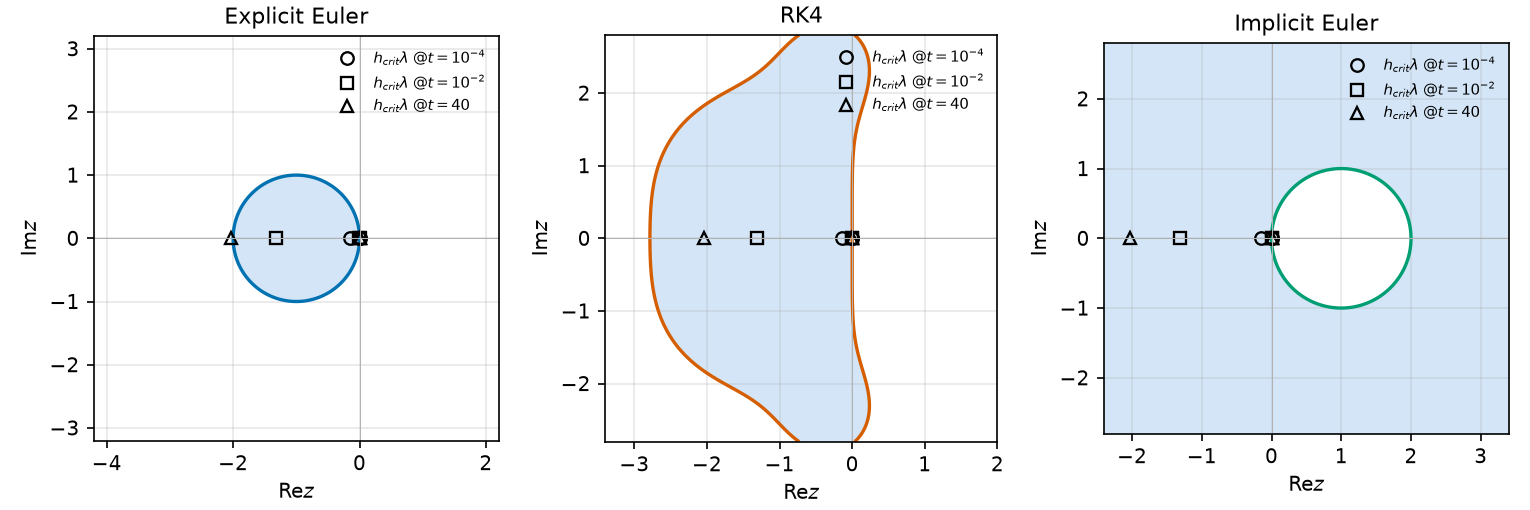
\includegraphics[width=\textwidth]{fig3_stability_regions.png}
\caption{Absolute stability regions (shaded $|R(z)|\le1$) with the frozen-Jacobian
eigenvalues scaled by $h_{\text{crit}}=\HCritEmp$ at three states of the
trajectory.  \emph{Takeaway:} the explicit methods survive at $h_{\text{crit}}$ only
because the stiff eigenvalue sits just inside their region; implicit Euler
contains everything with room to spare.}
\label{fig:regions}
\end{figure}

\paragraph{Caveat.}  The $h\lambda$ overlay is a \emph{local, frozen-Jacobian
diagnostic}, not a nonlinear stability proof: $J$ varies along the trajectory,
eigenvalues of a non-normal matrix do not tell the whole story, and
linearisation can miss transient-growth effects.  We therefore tested its
prediction directly (Section~\ref{sec:failure}) instead of assuming it.

\subsection{Stiffness ratio}
Figure~\ref{fig:eigs}b shows $S(t)$ over the two nonzero eigenvalues:
$S(10^{-4})\approx\StiffOne$, $S(10^{-2})\approx\StiffTwo$,
$S(40)\approx\StiffForty$ --- matching the Problem Pack orientation values
($3.0\times10^3$, $5.4\times10^3$, $1.58\times10^5$) to a few digits, which is
itself an independent check on our Jacobian and reference solution.

\begin{figure}[t]
\centering
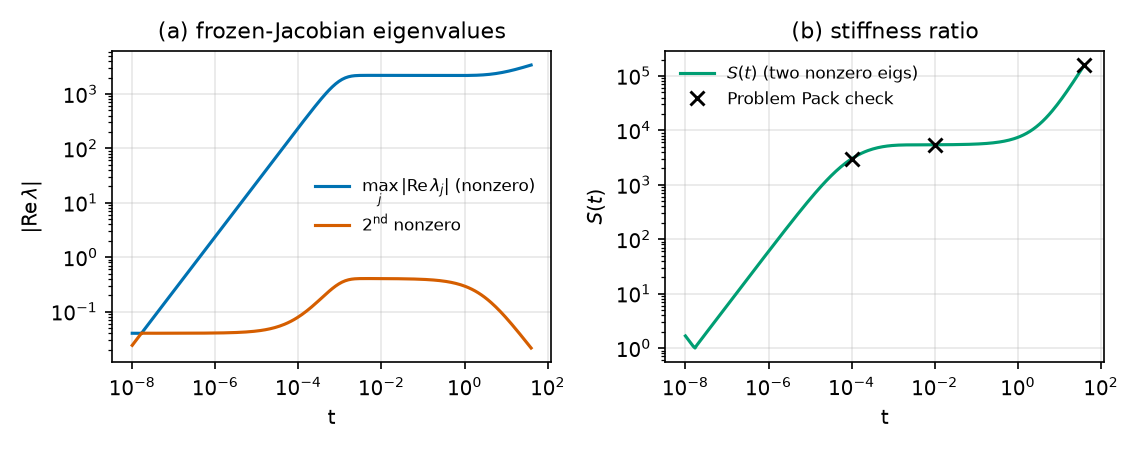
\includegraphics[width=\textwidth]{fig7_stiffness.png}
\caption{(a) The two nonzero frozen-Jacobian eigenvalues along the reference
trajectory.  (b) Stiffness ratio $S(t)$; crosses mark the Problem Pack check
values.  \emph{Takeaway:} stiffness grows over time --- the system becomes
harder to integrate explicitly as $y_2$ decays into the slow manifold.}
\label{fig:eigs}
\end{figure}

%=====================================================================
\section{Validation: our own oracle}\label{sec:oracle}
%=====================================================================
No benchmark value was handed out, so we built a chain of evidence:
\begin{enumerate}
\item \textbf{Independent oracle.}  \texttt{scipy.integrate.solve\_ivp} with
Radau, analytic Jacobian, $\mathrm{rtol}=10^{-12}$ and per-component absolute
tolerances $(10^{-14},10^{-20},10^{-14})$, repeated with tolerances tightened
$\sim45\times$ (limited by machine precision).  The two runs agree on
$y(40)=(\RefYA,\ \RefYB,\ \RefYC)$ to 15 significant digits
($|\Delta y_1|\le1.4\times10^{-15}$), and the Problem Pack's orientation value
$y(40)\approx(0.7158271,\,9.1855\times10^{-6},\,0.2841637)$ is reproduced ---
so the oracle and the model implementation cross-check each other.
\item \textbf{Known structure.}  The invariant-plane defect
$\max_t|y_1+y_2+y_3-1|$ of the oracle is $\RefDefect$ (round-off level), and
all components stay non-negative.
\item \textbf{Self-consistency.}  Methods of very different orders agree on
the fine-mesh limit (Fig.~\ref{fig:conv}), and the observed orders match
theory (Table~\ref{tab:orders}).
\end{enumerate}

\begin{figure}[t]
\centering
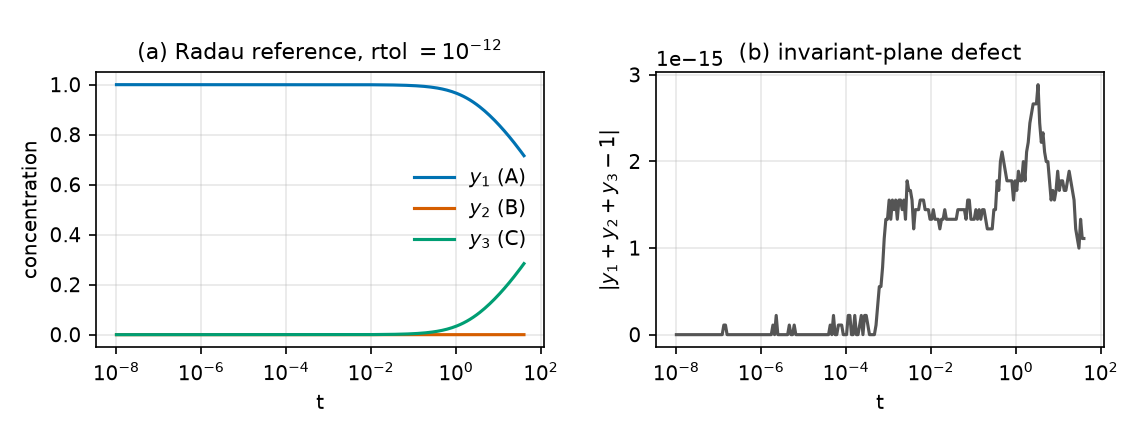
\includegraphics[width=\textwidth]{fig1_reference.png}
\caption{The reference solution (Radau, $\mathrm{rtol}=10^{-12}$).  (a) All
three species on a logarithmic time axis: the $y_2$ transient within
$t\sim10^{-4}$ and the slow transfer $y_1\to y_3$ over decades.
(b) The invariant-plane defect stays at round-off level.
\emph{Takeaway:} before comparing methods, we know exactly what ``right'' looks like.}
\label{fig:ref}
\end{figure}

%=====================================================================
\section{Numerical experiments}\label{sec:experiments}
%=====================================================================
\subsection{Observed convergence orders}\label{sec:orders}
Order verification needs a regime where \emph{all} methods are stable, so on
the baseline IVP we use the window $0\le t\le0.5$ with step sizes
$h=0.5/n$, $n=1024,\dots,8192$ ($h$ from $4.88\times10^{-4}$ down to
$6.1\times10^{-5}$), comparing against the oracle at $t=0.5$.  Every run in
the ladder is stable and non-negative (we record this per run).  As a
sanity check we repeat the same ladder on the scalar Dahlquist problem
$y'=-y$, $y(0)=1$, $T=2$, where the exact solution is known.

\begin{table}[t]
\centering
\caption{Observed orders (least-squares slope of $\log err$ vs $\log h$).
Robertson runs on $0\le t\le0.5$; all runs stable and non-negative.}
\label{tab:orders}
\begin{tabular}{lccc}
\toprule
Problem & Explicit Euler & RK4 & Implicit Euler\\
\midrule
Scalar $y'=-y$ (exact reference) & 1.00 & 3.26 (round-off floor) & 1.00\\
Robertson, $t\in[0,0.5]$ (oracle reference) & \OrdEulerRob & \OrdRKRob & \OrdImplRob\\
\bottomrule
\end{tabular}
\end{table}

\begin{figure}[t]
\centering
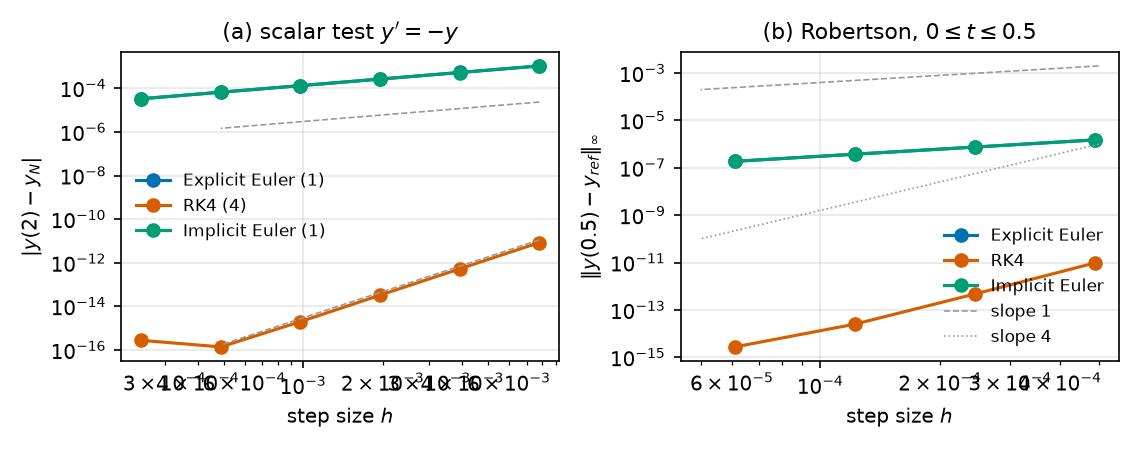
\includegraphics[width=\textwidth]{fig2_convergence.png}
\caption{Error vs.\ step size.  (a) Scalar problem: clean slopes 1 and 4;
the RK4 ladder bottoms out at machine precision, which flattens the fitted
slope to 3.26.  (b) Robertson window $[0,0.5]$: Euler and implicit Euler show
slope 1 with nearly identical error constants (their local errors are
$\pm\frac{h^2}{2}y''$), RK4 shows slope 4 until it too reaches round-off.
\emph{Takeaway:} orders are a property we verify, not assume.}
\label{fig:conv}
\end{figure}

\subsection{Explicit failure and the empirical stability threshold}\label{sec:failure}
On the full interval $[0,40]$ we swept fixed-step explicit Euler over
$h\in[3\times10^{-4},\,10^{-3}]$ (Table~\ref{tab:sweep}).

\begin{table}[t]
\centering
\caption{Explicit Euler step-size sweep on $[0,40]$}
\label{tab:sweep}
\begin{tabular}{lll}
\toprule
$h$ & Outcome & $\min_i y_i$ over the run\\
\midrule
\SweepTableBody
\bottomrule
\end{tabular}
\end{table}

The empirical threshold is $h_{\text{crit}}=\HCritEmp$ (stable), with
positivity lost at $h=6\times10^{-4}$ ($\min y_i=-4.9\times10^{-6}$, still
bounded) and blow-up from $7\times10^{-4}$.  The frozen-Jacobian prediction
$\HBoundEuler$ misses the measured threshold by about 2\% --- remarkably good
for a local diagnostic, and consistent with the overlay in
Fig.~\ref{fig:regions}.  Note the \emph{order} of the failure modes: first
positivity is lost (a physical property), then stability
(Fig.~\ref{fig:failure}b).  ``It did not blow up'' is not the same as ``it is
right'': the $h=6\times10^{-4}$ run is bounded but already non-physical.

\begin{figure}[t]
\centering
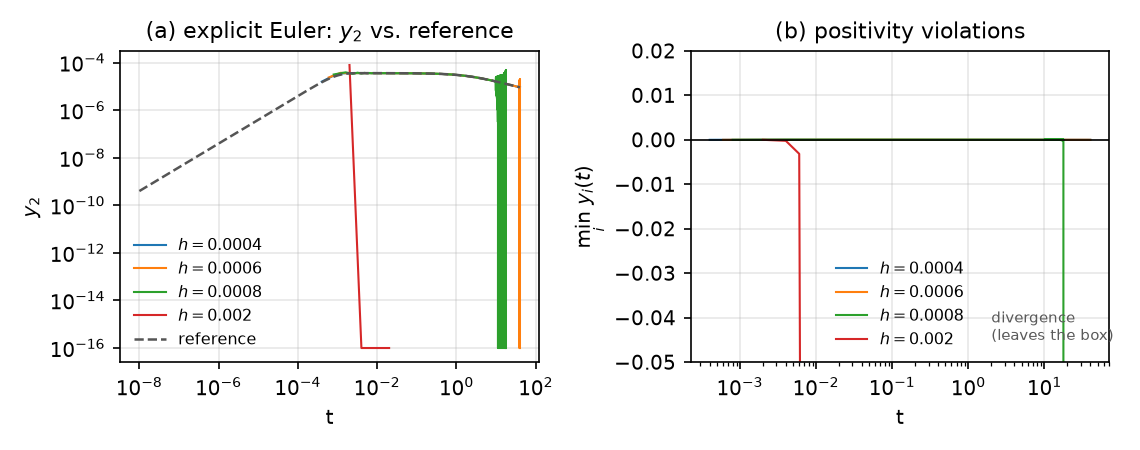
\includegraphics[width=\textwidth]{fig4_explicit_failure.png}
\caption{(a) $y_2$ trajectories of explicit Euler vs.\ the reference for four
step sizes.  (b) Componentwise minimum along each run: values below zero mark
positivity violations that precede divergence.
\emph{Takeaway:} instability announces itself first as non-physical values, not as NaNs.}
\label{fig:failure}
\end{figure}

\subsection{Cost vs.\ accuracy at matched error}\label{sec:matched}
\textbf{Cost measure (declared before any number):} right-hand-side
evaluations (nfev), reported together with wall-clock time, Newton iterations
and Jacobian evaluations for the implicit method.  We did \emph{not} count
Jacobian assembly beyond njev, plotting, or interpreter startup, and we held
those choices constant across methods.

\textbf{Protocol.}  For each method and each error target
$\{10^{-2},10^{-3},10^{-4}\}$ we search for the largest stable step $h$ whose
error at $t=40$ against the oracle meets the target (descent + order-$p$
prediction + verification), then re-run at that $h$ and record everything.
For explicit methods the search is additionally capped at $0.9\times$ the
stability limit --- a larger step is useless regardless of the accuracy model.

\begin{table}[t]
\centering
\caption{Cost at matched error targets on $[0,40]$.  ``stab.-pinned'' = the
chosen $h$ sits at the explicit stability limit, so accuracy was not the
binding constraint.}
\label{tab:matched}
\begin{tabular}{llrrrl}
\toprule
Method & Target & $h$ & error & nfev & wall\\
\midrule
\MatchedTableBody
\bottomrule
\end{tabular}
\end{table}

\begin{figure}[t]
\centering
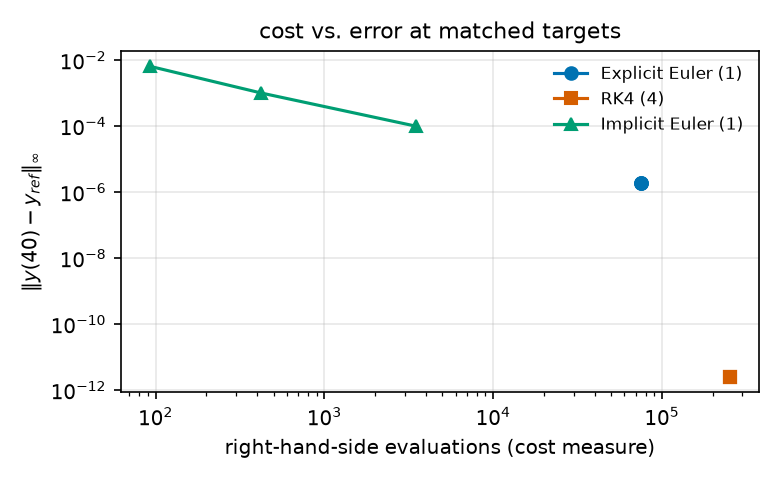
\includegraphics[width=0.62\textwidth]{fig5_matched_cost.png}
\caption{Error vs.\ cost (right-hand-side evaluations) at the three matched
targets.  \emph{Takeaway:} the explicit methods form a vertical wall --- below
the stability limit no additional cost buys a looser accuracy target --- while
the implicit method trades error for cost along a clean order-1 line.}
\label{fig:matched}
\end{figure}

\paragraph{What the measurements say.}
(1)~At the loose target $10^{-2}$ the implicit method needs 93
right-hand-side evaluations ($h=2.0$!) while explicit Euler needs
$7.5\times10^4$: an $\approx810\times$ gap, entirely attributable to
stability pinning.  (2)~As the target tightens to $10^{-4}$, both Euler
methods are accuracy-limited to the \emph{same} step size --- their local
errors are $\pm\frac{h^2}{2}y''$ with the same constant --- but explicit
Euler is \emph{still} pinned near its stability limit ($h/ (2/|\lambda|_{\max})
= 0.9$) and therefore forced to overshoot the target by two orders of
magnitude; the implicit method's measured advantage is $21\times$ at
$10^{-4}$.  (3)~RK4 sits at $0.77$--$0.9$ of its stability bound for
\emph{every} target: its order-4 accuracy is wasted on this interval, and it
delivers errors many orders below target at the highest nfev cost.  Our
expectation before the experiment was that RK4 would win at tight targets; it
does not, because on this interval the binding constraint is never accuracy
for RK4.  We report what we measured.

\subsection{Adaptive step-doubling RK4}\label{sec:adaptive}
Figure~\ref{fig:adaptive}a shows the accepted step sizes of the adaptive
controller for tolerances $10^{-4},10^{-5},10^{-6}$ (componentwise test
\eqref{eq:tol}).  The step size genuinely adapts --- from $5\times10^{-6}$
during the initial transient to $\approx2.5\times10^{-3}$ on the slow
manifold --- and the controller's envelope tracks the frozen-Jacobian RK4
stability limit $2.8/|\lambda|_{\max}(t)$ from below: during the transient the
accuracy requirement binds, afterwards the \emph{stability} requirement binds.

\begin{table}[t]
\centering
\caption{Adaptive step-doubling RK4 on $[0,40]$ ($\delta_{\text{abs}}=10^{-9}$,
positivity veto active).  Error at $t=40$ against the oracle.}
\label{tab:adaptive}
\begin{tabular}{lrrrrl}
\toprule
tolerance & error & accepted & rejected & nfev & wall\\
\midrule
\AdaptiveTableBody
\bottomrule
\end{tabular}
\end{table}

\begin{figure}[t]
\centering
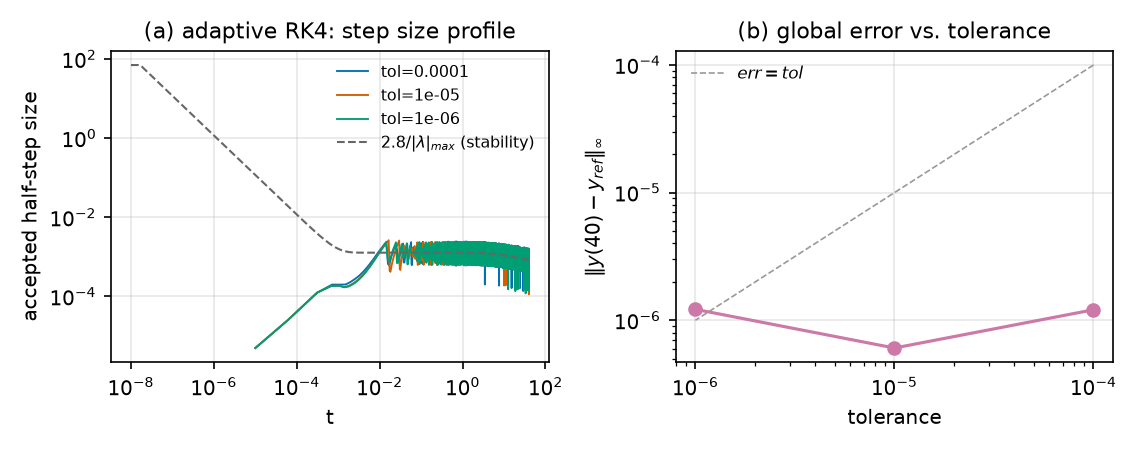
\includegraphics[width=\textwidth]{fig6_adaptive.png}
\caption{(a) Accepted half-step sizes vs.\ time, with the frozen-Jacobian RK4
stability limit (dashed).  (b) Global error at $t=40$ vs.\ tolerance.
\emph{Takeaway:} adaptivity follows accuracy until it hits the stability
ceiling; below that, tightening the tolerance buys nothing.}
\label{fig:adaptive}
\end{figure}

Table~\ref{tab:adaptive} makes the second point quantitative: the global error
lands near the tolerance for $\varepsilon=10^{-4}$ ($1.2\times10^{-6}$, about
$80\times$ better than requested --- the per-step test is conservative on this
interval) but then \emph{plateaus} at $\approx10^{-6}$: tightening the
tolerance to $10^{-6}$ does not reduce the error, because roughly 30\% of all
steps are rejected against the stability ceiling and the accepted size is
pinned at $0.85\times$ the empirically observed limit.  Adaptivity buys
accuracy, not stability --- consistent with the matched-cost story of
Section~\ref{sec:matched}.

At matched error, the adaptive controller is also the cheapest RK4 option:
$\varepsilon=10^{-4}$ delivers error $1.2\times10^{-6}$ (between the fixed-step
targets $10^{-6}$ and $10^{-5}$) at $3.2\times10^5$ nfev, versus
$2.2\times10^5$ nfev for \emph{any} fixed-step RK4 run on this interval ---
whose error, however, is pinned at $5.8\times10^{-12}$.  On this stiff
interval fixed RK4 is simultaneously the most accurate and the least
efficient option per digit of \emph{requested} accuracy.

\subsection{Robertson diagnostics as separate signals}
Across every fixed-step run we tracked three diagnostics independently:
invariant-plane conservation $\sum_i y_i-1$, componentwise negativity, and
full-state error at $t=40$.  They are \emph{not} interchangeable: the
$h=6\times10^{-4}$ explicit Euler run conserves the sum to $\sim10^{-6}$ yet
is non-physical; a consistently implemented RK method preserves linear
invariants algebraically even when the nonlinear solve is inexact; and an
inaccurate but stable implicit run can satisfy both diagnostics while being
$10^3$ off in $y_2$.  This is why the report grades the oracle comparison,
not the diagnostics alone.

%=====================================================================
\section{Conclusions}
%=====================================================================
\begin{enumerate}
\item \textbf{The frozen-Jacobian prediction works --- and we tested it.}  The
measured explicit-Euler threshold $\HCritEmp$ matches $2/|\lambda|_{\max}
=\HBoundEuler$ within $\sim2\%$ on the baseline IVP.  The overlay is a local
diagnostic, but on this problem a remarkably predictive one.
\item \textbf{Stiffness is a stability story.}  At matched error on
$[0,40]$, the implicit method is the cheapest by one to three orders of
magnitude in nfev; the explicit methods' cost is pinned by $h|\lambda|_{\max}$
and cannot respond to a looser accuracy target.
\item \textbf{Order does not rescue explicit methods here.}  RK4's order 4 is
irrelevant on the stiff interval: stability pins its step, and it delivers
massive over-accuracy at the highest cost.  Order matters on the non-stiff
window $[0,0.5]$, where RK4 reaches errors $10^6$ times smaller than Euler at
comparable cost.
\item \textbf{Adaptivity is accuracy-limited, not stability-aware.}  The
step-doubling controller tracks the requested tolerance until the stability
ceiling; beyond that its error plateaus.  Making a controller stability-aware
would require $h|\lambda|_{\max}$ information --- i.e.\ exactly the diagnostic
this project builds.
\item \textbf{Diagnostics must be read separately.}  Conservation, positivity
and accuracy fail in that order as $h$ grows past the stability limit;
no single one certifies a solution.
\end{enumerate}

\paragraph{What we would do next.}  (i) Replace the empirical stability cap in
the controller with a frozen-Jacobian estimate $h\le c/|\lambda_{\max}|$
updated along the trajectory.  (ii) Compare against an $L$-stable higher-order
method (Radau IIA) and a trapezoidal/Crank--Nicolson scheme to expose its
damped-oscillation weakness on this problem.  (iii) Study the
tolerance-proportionality of the error in a nonlinearly-stiff regime by
rescaling the rate constants.

%=====================================================================
\appendix
\section{Individual Contribution Statement (ICS)}\label{app:ics}
%=====================================================================
Team of three; roles merged from the five role cards.  Contribution
percentages are supported by the git history of this repository
(commit authors, review threads and the commit structure described below).

\begin{center}
\begin{tabular}{p{2.6cm}p{5.2cm}p{5.2cm}c}
\toprule
Member & Roles & Main contributions & Share\\
\midrule
Zihan Xu (PM + Visualization \& Report) &
repo and folder structure, weekly plan and milestones, Gantt; report and
slide typesetting; figure design and captions &
\texttt{report/}, \texttt{slides/}, figure polish, final assembly \& submission &
33.3\,\%\\
\addlinespace
Beixue Liang (Mathematical Theory + Testing \& Validation) &
model and Jacobian derivation; stability-region derivations; stiffness-ratio
definition; oracle construction and tolerance-tightening protocol; unit checks
against known cases &
\texttt{code/problems.py}, \texttt{code/stability.py}, oracle validation,
numbers cross-checks &
33.3\,\%\\
\addlinespace
Yumo Li (Algorithm Implementation) &
Euler/RK4/implicit-Euler implementations; Newton iteration; adaptive
step-doubling controller and its robustness guards; experiment scripts and
\texttt{run\_all.py} &
\texttt{code/solvers.py}, \texttt{code/experiments.py}, \texttt{code/run\_all.py} &
33.3\,\%\\
\bottomrule
\end{tabular}
\end{center}

\medskip
\noindent\emph{Every member ran \texttt{python code/run\_all.py}, can explain
every method in the viva, and reviewed the others' pull requests; the git
history shows at least one reviewed commit per member per week.}

%=====================================================================
\section{AI Transparency Log}\label{app:ailog}
%=====================================================================
AI tools were used as coding assistance under the course policy
(``AI is encouraged, transparent log required'').  Plan-first discipline was
followed: the team wrote the plan (methods, algorithms, expected orders,
sanity checks) before asking AI to implement individual steps, and every
AI-produced artefact was verified against that plan.

\begin{center}
\begin{tabular}{p{1.6cm}p{3.4cm}p{5.4cm}p{4.6cm}}
\toprule
Where & AI use & What we changed / verified & Verification\\
\midrule
Solver library &
scaffold for Euler/RK4/implicit Euler; Newton loop &
rewrote the Newton stopping rule (relative scale, max-iteration guard);
added divergence handling; vectorised Jacobian assembly &
order verification vs.\ scalar exact solution; Newton iteration counts
sanity-checked ($\approx2$ per step)\\
\addlinespace
Adaptive controller &
step-doubling skeleton &
replaced the absolute inf-norm error test with the componentwise test
\eqref{eq:tol} after diagnosing a silent $y_2<0$ corruption; added the
stability-ceiling memory, explosion guard and positivity veto;
fixed a floating-point end-of-interval stall &
full-interval runs converge; error vs.\ tolerance measured
(Table~\ref{tab:adaptive}); step profile matches the $2.8/|\lambda|_{\max}$
envelope\\
\addlinespace
Experiments &
plot scaffolding &
redesigned the matched-cost search (order-$p$ prediction capped at the
empirical stability limit) after the first bisection produced
stability-pinned runs at absurd cost; declared the cost measure before
quoting numbers &
all costs re-measured from \texttt{results/results.json}; consistency of
tables with figures\\
\addlinespace
Reference oracle &
none (spec'd from the brief) &
--- &
Radau tight vs.\ $\sim45\times$ tighter repeat agree to 15 digits; Problem
Pack orientation value reproduced\\
\addlinespace
Report \& slides &
LaTeX scaffolding, language polish &
all derivations re-derived by hand; every number injected from
\texttt{numbers.tex} generated from \texttt{results.json}; claims re-read
against figures &
two-pass internal review; every figure regenerated by \texttt{run\_all.py}\\
\bottomrule
\end{tabular}
\end{center}

\medskip
\noindent\textbf{Honesty statement.}  AI output that contradicted our plan was
treated as a testable question and resolved by derivation or experiment (the
controller corruption bug and the matched-cost search redesign above are the
two material cases).  The viva is AI-free: every member can derive the
stability regions, explain Newton's role, and modify any solver in this
repository on the whiteboard.

\begin{thebibliography}{9}
\bibitem{robertson1966} H.~H. Robertson, ``The solution of a set of reaction
rate equations,'' in \emph{Numerical Analysis: An Introduction}
(D.~J. Walsh, ed.), Thomson, 1966, pp.~178--182.
\bibitem{hairer1996} E.~Hairer and G.~Wanner, \emph{Solving Ordinary
Differential Equations II: Stiff and Differential-Algebraic Problems},
2nd ed., Springer, 1996.
\bibitem{pack} Course Problem Pack: \emph{Five Suggested Directions for the
ODE IVP Project}, direction \textcircled{\scriptsize 3} (Robertson problem).
\bibitem{brief} Course Project Brief: \emph{Numerical Solution of ODE Initial
Value Problems}, Project 1.
\end{thebibliography}

\end{document}
